\documentclass[10pt,aspectratio=169]{beamer}
\usepackage{tikz}
\usetheme{Boadilla}
\setbeamertemplate{navigation symbols}{}
\title{Iterative refinement: experiments and bounds}
\subtitle{Generated interaction study}
\author{Research group}
\date{}
\year=2026\month=11\day=5
\newcommand{\fuzzlayerA}[1]{\textbf{#1}}
\newcommand{\fuzzlayerB}[1]{\fuzzlayerA{#1}}
\newcommand{\fuzzterm}[1]{\fuzzlayerB{#1}}
\newcommand{\fuzzpair}[2]{\fuzzterm{#1}: #2}
\newcommand{\fuzzunit}{Hz}
\let\fuzzoriginalunit\fuzzunit
\newcommand{\fuzzcoefficient}{2}
\newcommand{\fuzzscale}[2][\fuzzcoefficient]{#1\,#2}
\definecolor{fuzzpaint}{RGB}{255,0,255}
\definecolor{fuzzsecond}{RGB}{18,137,67}
\tikzset{fuzzvertex/.style={draw,rounded corners=1pt,fill=blue!10,inner sep=1pt,minimum width=.35cm,minimum height=.25cm}}
\begin{document}
\section{Iterative refinement}
\begin{frame}[t,shrink=5]{Iterative refinement}{Composed dependencies}
\fuzzpair{Experiment}{Timing: 12\fuzzunit; estimate $\fuzzscale{x}+\fuzzscale[2]{y}$.}\par
{\renewcommand{\fuzzunit}{cycles}\let\fuzzterm\textrm\fuzzpair{LocalScope}{Timing: 7\fuzzunit.}\par}
\fuzzpair{RestoredScope}{Timing: 11\fuzzunit.}\par
\begin{columns}[onlytextwidth,t]
\begin{column}{0.38\textwidth}
\begin{columns}[onlytextwidth,c]
\begin{column}{0.38\textwidth}
\textrm{The final diagram} records the order in which information crosses the partition.  The estimate is $\frac{a+b}{1+c}$.
\par
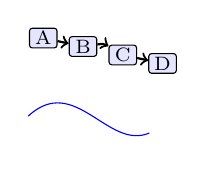
\begin{tikzpicture}[font=\scriptsize]
\begin{scope}[scale=1.1,rotate=-12]


\node[fuzzvertex] (g4n0) at (0.000,0) {A};
\node[fuzzvertex] (g4n1) at (0.469,0) {B};
\node[fuzzvertex] (g4n2) at (0.939,0) {C};
\node[fuzzvertex] (g4n3) at (1.408,0) {D};
\begin{scope}[xshift=.5pt,yshift=-.5pt]
\draw<2->[->,thick] (g4n0) -- (g4n1);
\draw<2->[->,thick] (g4n1) to[bend left=20] (g4n2);
\draw<2->[->,thick] (g4n2) -- (g4n3);
\draw[blue] (0,-.9) .. controls (0.422,-.3) and (0.986,-1.1) .. (1.408,-.8);
\end{scope}
\end{scope}
\end{tikzpicture}
\end{column}
\begin{column}{0.58\textwidth}
\begin{itemize}
\item<1-> \begin{tikzpicture}\node[draw] {
\includegraphics[scale=.75]{fuzz-images/pattern.v2}};\end{tikzpicture}
\item<2-> \[\begin{aligned}a+b&=c\\ d-e&=f\end{aligned}\]
\par
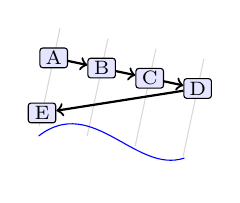
\begin{tikzpicture}[font=\scriptsize]
\begin{scope}[scale=1.1,rotate=-12]

\foreach \x in {0,1,2,3} {\draw[gray!30] (\x*0.566,-.8)--(\x*0.566,.35);}
\node[fuzzvertex] (g9n0) at (0.000,0) {A};
\node[fuzzvertex] (g9n1) at (0.566,0) {B};
\node[fuzzvertex] (g9n2) at (1.133,0) {C};
\node[fuzzvertex] (g9n3) at (1.699,0) {D};
\node[fuzzvertex] (g9n4) at (0.000,-0.65) {E};
\begin{scope}[xshift=.5pt,yshift=-.5pt]
\draw<2->[->,thick] (g9n0) -- (g9n1);
\draw<2->[->,thick] (g9n1) -- (g9n2);
\draw<2->[->,thick] (g9n2) -- (g9n3);
\draw<2->[->,thick] (g9n3) -- (g9n4);
\draw[blue] (0,-.9) .. controls (0.510,-.3) and (1.189,-1.1) .. (1.699,-.8);
\end{scope}
\end{scope}
\end{tikzpicture}
\end{itemize}
\end{column}
\end{columns}
\end{column}
\begin{column}{0.58\textwidth}
\begin{description}
\item[Stage 1] \begin{columns}[onlytextwidth,c]
\begin{column}{0.62\textwidth}
Before 
\includegraphics[viewport=1 1 20 14,clip]{fuzz-images/pattern.png} after.
\end{column}
\begin{column}{0.34\textwidth}
\begin{description}
\item<1->[Stage 1] \[E=\sum_{i=1}^{n}w_i x_i\]
\end{description}
\end{column}
\end{columns}
\item[Stage 2] \begin{columns}[onlytextwidth,t]
\begin{column}{0.54\textwidth}
\textbf{The next pass} must preserve the boundary conditions while revisiting dependent values.  The estimate is $x_i+x_{i+1}$.
\end{column}
\begin{column}{0.42\textwidth}
\textit{A local update} can change the measurements used by several neighboring components.  The estimate is $\alpha+\beta$.
\end{column}
\end{columns}
\item[Stage 3] \begin{center}
Before 
\includegraphics[page=2,origin=c,angle=-30,totalheight=18pt]{fuzz-images/pages.pdf} after.
\end{center}
\end{description}
\end{column}
\end{columns}
\par 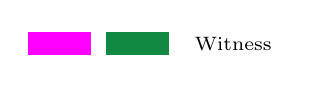
\begin{tikzpicture}[font=\scriptsize]
\fill<2-3>[fuzzpaint] (0,0) rectangle (.8,.3);
\fill<3->[fuzzsecond] (1,0) rectangle (1.8,.3);
\node[anchor=west] at (2,0.15) {Witness};
\end{tikzpicture}
\only<4>{}
\end{frame}
\renewcommand{\fuzzunit}{min}
\renewcommand{\fuzzcoefficient}{2}
\renewcommand{\fuzzterm}[1]{{\textit{#1}}}
\section{Message passing}
\begin{frame}[t]{Constraint propagation}
\fuzzpair{MacroStageB}{Timing: 12\fuzzunit, retained: 9\fuzzoriginalunit.}\par
{\renewcommand{\fuzzunit}{local}\fuzzpair{FrameLocal}{Timing: 5\fuzzunit.}\par}
\fuzzpair{FrameRestored}{Timing: 8\fuzzunit; estimate $\fuzzscale{x}$.}\par
\begin{columns}[T]\begin{column}{.46\textwidth}The final diagram records the order in which information crosses the partition.\end{column}\begin{column}{.46\textwidth}\begin{itemize}\item Input state\item Updated state\end{itemize}\end{column}\end{columns}
\end{frame}
\renewcommand{\fuzzunit}{steps}
\renewcommand{\fuzzcoefficient}{3}
\renewcommand{\fuzzterm}[1]{{\textit{#1}}}
\section{Iterative refinement}
\begin{frame}[t]{Incremental analysis}
\fuzzpair{MacroStageC}{Timing: 12\fuzzunit, retained: 9\fuzzoriginalunit.}\par
{\renewcommand{\fuzzunit}{local}\fuzzpair{FrameLocal}{Timing: 5\fuzzunit.}\par}
\fuzzpair{FrameRestored}{Timing: 8\fuzzunit; estimate $\fuzzscale{x}$.}\par
\begin{block}{Follow-up}\fuzzterm{A revised value} depends on the preceding frame.\end{block}
\[r_{k+1}=r_k-\alpha d_k\]
\end{frame}
\renewcommand{\fuzzunit}{s}
\renewcommand{\fuzzcoefficient}{4}
\renewcommand{\fuzzterm}[1]{{\textit{#1}}}
\section{Cache invalidation}
\begin{frame}[t]{Incremental analysis}
\fuzzpair{MacroStageD}{Timing: 12\fuzzunit, retained: 9\fuzzoriginalunit.}\par
{\renewcommand{\fuzzunit}{local}\fuzzpair{FrameLocal}{Timing: 5\fuzzunit.}\par}
\fuzzpair{FrameRestored}{Timing: 8\fuzzunit; estimate $\fuzzscale{x}$.}\par
\begin{columns}[T]\begin{column}{.46\textwidth}The final diagram records the order in which information crosses the partition.\end{column}\begin{column}{.46\textwidth}\begin{itemize}\item Input state\item Updated state\end{itemize}\end{column}\end{columns}
\end{frame}
\end{document}
